% Template for PLoS (Adapted for Frontiers, MdK))
% Version 1.0 January 2009
%
% To compile to pdf, run:
% latex plos.template
% bibtex plos.template
% latex plos.template
% latex plos.template
% dvipdf plos.template

\documentclass[12pt]{article}

% amsmath package, useful for mathematical formulas
\usepackage{amsmath}
% amssymb package, useful for mathematical symbols
\usepackage{amssymb}

% graphicx package, useful for including eps and pdf graphics
% include graphics with the command \includegraphics
\usepackage{graphicx}

% cite package, to clean up citations in the main text. Do not remove.
\usepackage{natbib}
\usepackage{cite}
\usepackage{lineno}
\usepackage{color} 

% Use doublespacing - comment out for single spacing
%\usepackage{setspace} 
%\doublespacing

% Text layout
\topmargin 0.0cm
\oddsidemargin 0.5cm
\evensidemargin 0.5cm
\textwidth 16cm 
\textheight 21cm

% Bold the 'Figure #' in the caption and separate it with a period
% Captions will be left justified
\usepackage[labelfont=bf,labelsep=period,justification=raggedright]{caption}

% Use the Frontiers provided bibtex style

% Remove brackets from numbering in List of References
%\makeatletter
%\renewcommand{\@biblabel}[1]{\quad#1.}
%\makeatother


% Leave date blank
\date{}

\pagestyle{myheadings}
%% ** EDIT HERE **

% the subfigure package
\usepackage{caption}
\usepackage{subcaption}

\DeclareCaptionFormat{subfig}{\figurename~#1#2#3}
\DeclareCaptionSubType*{figure}
\captionsetup[subfigure]{format=subfig,labelsep=colon,labelformat=simple}

% the listings package
\usepackage{listings}
\lstset{
language=C++,
basicstyle=\footnotesize,
numbers=right,
numberstyle=\tiny,
frame=tb,
columns=fullflexible,
showstringspaces=false
}


%% ** EDIT HERE **
%% PLEASE INCLUDE ALL MACROS BELOW

%% END MACROS SECTION

\begin{document}

% Title must be 150 characters or less
\begin{center}
\thispagestyle{empty}
{\Large
\textbf{Parallel MIIND: a Parallel Framework for Populations of Spiking Neurons Using Population Density Techniques}
}
\vspace{1.0cm}
% Insert Author names, affiliations and corresponding author email.
\\
Marc de Kamps$^{1,\ast}$, 
David Sichau$^{2}$
\vspace{0.5cm}
\\
\bf{1} School of Computing, University of Leeds, Leeds, West Yorkshire, UK
\\
\bf{2} David's address
\\
\vspace{0.5cm}
$\ast$ E-mail: m.dekamps@leeds.ac.uk
\end{center}

% Please keep the abstract between 250 and 300 words
\section*{Abstract}


%\section*{Author Summary}
\newpage 
\setcounter{page}{1}
\linenumbers

\section{Introduction}
Multiple Interacting Instantiations of Neural Dynamics \citep{dekamps2008} (MIIND) is a simulation framework designed for modeling large networks of 
neuronal populations. It is written in C++ and employs MPI \citep{gropp1998} for parallelisation. Python extensions can be provided on request. 
Due to its design philosophy it can be easily applied to modeling 
biological processes outside computational neuroscience. MIIND abstracts the interaction between neuronal populations into an interaction 
between nodes on a directed graph. The neuronal processes describing the activity of the population live on these nodes as objects and evolve 
the population’s state. In general we aim to support network processes that use CPU-intensive computations to model nodes, but
require little bandwidth in the internode communication. Neuronal networks where individual spikes are less important than the transmission
of population firing rates are well supported by this paradigm. As such, the processes that are supported by this framework are trivially
parallelizable. Unfortunately, the word trivial does not apply to the actual implementation: we found that in the original code base of MIIND there
were too many obstacles to parallelisation and we decided to start from a fresh code based. 

As with any framework, MIIND comes with a number of predefined algorithms, some allowing sophisticated simulations of neuronal 
dynamics. The simplest algorithms implement Wilson-Cowan dynamics \citep{wilson1972}, but, uniquely, 
MIIND provides an implementation of population density techniques (e.g.) \citep{stein1965,knight1972,knight1996}. They provide efficient simulations 
of large populations of neurons by means of a density function over the state variables of a given neuron. Such techniques have undergone rapid 
development over the last decade \citep{omurtag2000}. In practice these techniques have been mainly used for leaky-integrate-and-fire (LIF) neurons,
in the so-called diffusion limit: small synaptic efficacies and high firing rate. In  this limit the distribution of membrane potentials of the
population can be modeled by a diffusion process, using Fokker-Planck equations. 

Recent progress has extended the usefulness of these technique considerably.  First, the techniques are no longer restricted to the diffusion limit 
\citep{omurtag2000,dekamps2003,dekamps2006}, indeed arbitrary large efficacies can be used.  Second, they are no longer restricted to LIF neurons: 
a method to model any one-dimensional neuronal model was described recently \citep{dekamps2013}, and will soon be part of the code base.
Others have described density approaches based on 2D neuronal models, including synaptic kinetics, and have established that networks
of 2D populations are computationally still competitive, compared to direct simulation.
  
The methods described here are at least an order of magnitude more efficient than direct simulation (a real second for a population of LIF neurons
can be modeled in well under 0.5 s simulated time \citep{dekamps2006}). Nevertheless, the computational load is such that a network of hundreds of such 
populations would lead to lengthy simulation runs on a serial machine. Therefore investigating the performance of such a network provides a good
benchmark for the scalability of the parallelisation approach.



% Results and Discussion can be combined.
\section{Results}
\subsection{The Framework}
In \citep{dekamps2008} we have outlined the general design ideas of the framework: populations can be modeled by nodes on a directed graph, 
which interact via the edges. The evolution of a population is determined by an Algorithm object which lives on the node and which maintains an 
AlgorithmGrid. A central simulation loop visits each node in term, collects the contributions from every other node connected to this node and calculates 
its input contribution weighted by the link value of the connection. Thus an instantaneous weighted input contribution from the entire network to node will 
be calculated, and this will be used by the algorithm to evolve its node state a small moment in time. This will result into an update of the AlgorithmGrid. 
By repeating this process for all nodes in the network for a desired period of time, a simulation of the network process is implemented. 
The central idea is represented in Figure 1. In the next section we will illustrate how network creation and configuring a simulation is done 
from the user's perspective.
\subsection{Simulating Networks as a Use Case}
Here we present a small program that performs a simulation of two neuronal populations: one excitatory and one inhibitory, driven by a common external input.
In listing \ref{code:twopopnet} the shortened code of this simulation is provided.
To increase the readability parameters are not provided. 
As a placeholder for the parameters the word PARAM is used.
Additional namespaces are ignored. 
For the whole program the reader is refered to the source code where this example is provided as \texttt{two-population.cpp}.
In the next section the setup of an simulation is explained step by step with the two population network.
\begin{lstlisting}[caption=Simulation of a two neuronal population network.,label=code:twopopnet]
int main(int argc, char* argv[]) {
#ifdef ENABLE_MPI
	boost::mpi::environment env(argc, argv);
#endif
	try {
		NodeId id_cortical_background;
		NodeId id_excitatory_main;
		NodeId id_inhibitory_main;
		MPINetwork<OrnsteinUhlenbeckConnection, CircularDistribution> network;

		// Create cortical background, and add to network
		populist::RateFunctor<WeightValue> cortical_background(PARAM);
		id_cortical_background = network.addNode(cortical_background, EXCITATORY);
		// Create excitatory main population
		PopulationAlgorithm_<OrnsteinUhlenbeckConnection> algorithm_excitatory(PARAM);
		id_excitatory_main = network.addNode(algorithm_excitatory, EXCITATORY);
		// Create inhibitory main population
		PopulationAlgorithm_<OrnsteinUhlenbeckConnection>  algorithm_inhibitory(PARAM);
		id_inhibitory_main = network.addNode(algorithm_inhibitory, INHIBITORY);

		// Background and excitatory connection only differ in x, 1- x
		network.makeFirstInputOfSecond(id_cortical_background, id_excitatory_main, PARAM);
		// Excitatory connection to itself
		network.makeFirstInputOfSecond(id_excitatory_main, id_excitatory_main, PARAM);
		// Background connection to I
		network.makeFirstInputOfSecond(id_cortical_background, id_inhibitory_main, PARAM);
		// E to I
		network.makeFirstInputOfSecond(id_excitatory_main, id_inhibitory_main, PARAM);
		// I to E
		network.makeFirstInputOfSecond(id_inhibitory_main, id_excitatory_main, PARAM);
		// I to I
		network.makeFirstInputOfSecond(id_inhibitory_main, id_inhibitory_main, PARAM);

		network.configureSimulation(PARAM);
		network.evolve();
	} catch (std::exception&e) {
		std::cout << e.what() << std::endl;
		return 1;
	}
	return 0;
}
\end{lstlisting}

For parallel MIIND it is important to initialise the mpi environment (see line 3 in listing \ref{code:twopopnet}).
To allow that the code is compilable without an mpi compiler the preprocessor is used to remove the code if mpi is not enabled.
These 3 lines are the only one where actually the user is forced to handle the mpi environment direct.
All other mpi related code is hidden from the user.

After the mpi environment is initialised one can start with setting up an simulation.
The network is created by instantiating a network object (line 9).
The network gets two template parameters.
The first parameter defines the connection type of the network.
In the example above this is a Ornstein Uhlenbeck type of connection.
The second parameter is the distribution of the nodes.
These parameter controls the distribution of the nodes in an mpi environment.
More details will be provided in the next section.

So far only the type of the network is defined.
To define the structure of the network two methods are needed.


The first method \texttt{addNode} adds a new nodes to the network (see line 13, 16 and 19).
This method expects the algorithm executed on this node and the type of the node.
In the example above 3 nodes are generated.
The cortical background driving the simulation with a constant firing rate (line 13).
And an excitatory and inhibitory node where leaky-integrate-and-fire neurons are simulated (line 16 and 19). %what reference for that

The method \texttt{addNode} returns the node id of the generated node.
The node ids start from 0 and are incremented by one for each additional nodes.
The order of the node ids correspond to the chronological order of the calls to \texttt{addNode}.
These ids are needed to identify the individual nodes and are needed for the second method to generate the network structure.

After the creation of the nodes the interactions of the network needs to be created.
Therefore directed connections between two nodes are generated.
Directed Connections between two nodes are generated by calling the method \texttt{makeFirstInputOfSecond}.
The method expects as parameters the node id of the first and the second node in the connection and the parameters of the connection (see line 22 - 32).
In the case of the two population network six connections are generated.
The background node is connected to the exhibitory and the inhibitory node.
The exhibitory and inhibitory nodes are connected to itself and to each other.
With these two methods the structure of the network is constructed.
The structure of the generated network can be seen in figure \ref{fig:twoPopNetwork}.

With these two methods all kind of networks can be generated.
To execute a simulation on that network the simulation needs to be configured.
The configuration is done by providing the simulation parameters to the method \texttt{configureSimulation} (see line 34 in listing \ref{code:twopopnet}).
When the simulation is configured the main simulation loop can be executed with the method \texttt{evolve}.

With the example provided above one can see that the generation of a simulation is straightforward.
It does not need any knowledge about the underlying parallelisation. More details about the parallelisation is provided in the next section.

\subsection{The Simulation Engine: An MPI-enabled Simulation Loop}%TODO(MdK) it is not only the simulation loop which is parallised. Maybe another title would be more suitable
In this section we will describe the mpi-based infrastructure that forms the heart of the framework.

To start with an illustration will be used.
A person wants to solve a large equation consiting of lot of different smaller equations.
In the beginning the person solved the equation on its own.
However it took a large amount of time for one person to solve the equations.
Therefore the management decided to hire additonal people to speed up the process.
To solve the equations faster each person needs to know what equation it should solve and sometimes the extension of another person equation is needed.
To share results and work they need to communicate with each other.
When people communicate with each other they cannot solve equations on the same time.
Additional the they might need lot of extensions of other people so they need to wait until the other people are finished with their calculation.
These two problems show some of the largest issues with parallelisation.
One is the overhead for communication.
And the other the latency.
The illustration above allegorize the message passing interface.

The Message passing interface mpi is a standard to develop applications aimed at large scale parallel applications.
An mpi program resembles an ordinary program written for a serial processor.
This similarity is deceptive, however.
In reallity the code is executed in parallel on different mpi processes.
A mpi process can be either executed on a single core of a multi core processor or on a different CPU.
These execution in different processes results that each process has its own memory space and not a shared memory space like a serial program.
That increases the amount of work to share data between the mpi processes.
For sharing data messages are sent between the individual mpi processes.
To send messages conncetions between the individual processes are needed.
The connections between the individual processes can be either a internal bus or a simple network connection.
However mpi is normally executed on super clusters with a very fast network connection (e.g. InfiniBand).

To speed-up a serial program with mpi the serial program is decomposed in parts that can be executed in parallel.
A serial program that is not embarrasing parallel results in data that needs to be shared between the mpi processes.
Therefore the individual mpi processes needs to communicate with each other to share the data.
To share the data between the mpi processes messages are sent from one mpi process to another with the data.
Compared to computation a message is very slow.
To reduce the overhead of parallelisation it is very important to reduce the number of messages to the minimum.


For the parallelisation of MIIND the idea was to distribute the nodes to MPI processes.
Each node can locally envole one time step without any communication.
The evolve step is responsible for most of the run time of an simulation the run time should be reduced by parallising these method.
To distribute the nodes to the mpi processes a distibution function is used.
As a default distribution function the circular distribution (\texttt{CircularDistribution}) is provided.
The circular distribution assignes the nodes in a circular manar to the mpi processes by using the modulor operator.
For example the network \ref{fig-realNetwork} would be represented internaly like \ref{fig-internalNetwork} when 4 mpi processes are available.
As the default distribution is not always the best choice it can be easily exchanged.
A new distribution can be implemented by implementing the virtual methods of the base class \texttt{NodeDistributionInterface}.
The implementation of a new distribution might be useful if another distribution would decrease the number of messages across the MPI processes (the dotted arrows in figure \ref{fig-internalNetwork}).
To implement a new distribution one might make use of additional knowledge of the network to decrease the messages over MPI process boarders.

With the distribution function the nodes are assigned to distinct mpi processes.
As the nodes are distributed over several mpi processes major changes inside the library where needed.

The parallelisation starts during the creation of the network.
When a node is added to the network the node is only generated on its responsible mpi process.
The method \texttt{addNode} is responsible for creating nodes.

\begin{lstlisting}[caption=The \texttt{addNode} method of the network.,label=code:addNode]
addNode(const AlgorithmInterface<WeightValue>& alg, NodeType nodeType) {
	NodeId tempNodeId = getMaxNodeId();
	if (nodeDistribution.isLocalNode(tempNodeId)) {
		MPINode node = MPINode(...);
		localNodes.insert(std::make_pair(tempNodeId, node));
	}
	incrementMaxNodeId();
	utilities::MPIProxy().barrier();
	return tempNodeId;
}
\end{lstlisting}

In listing \ref{code:addNode} the simplified method is provided.
The method starts with getting the next node id (see line 2 in listing \ref{code:addNode}.
The node id needs to be synchonised between the mpi processes to make sure that each nodes gets an unique id.
The ids of the nodes starts with 0 and increasing numbers are assigned to each node depending on the time of their initialization.
At this moment all mpi processes have the same node id.
To generate a node only on the responsibel mpi process the check on line 3 is carried out.
The \texttt{nodeDistribution} is the choosen distribution class, which checks if the node should be assigned to this mpi process.
If the node should generate on this node the node is generated and stored in the map \texttt{localNodes}, where the nodes on this mpi process are stored with their id as an key.
After the node is generated, or not the node id needs to be increased by calling the method \texttt{incrementMaxNodeId()}.
To avoid side effects the \texttt{addNode} method is synchronised.
For synchronous code mpi barriers are used which make sure that the function is only finished if all processes have executed all code.
As the generation of nodes happen only during the initialization this synchronous code has no impact on the performance.




As the mpi processes have different memory spaces the connections between the nodes cannot be stored anymore by connecting the nodes direct (via pointers or references).
The connections are generated by calls to the \texttt{makeFirstInputOfSecond} method.


\begin{lstlisting}[caption=The simplified \texttt{makeFirstInputOfSecond} method of the network.,label=code:makeFirstInputOfSecond]
makeFirstInputOfSecond(NodeId first, NodeId second, const WeightValue& weight) {
	//Make sure that the node exists and then add the successor
	if (nodeDistribution.isLocalNode(first)) {
		localNodes.find(first)->second.addSuccessor(second);
	}
	// Make sure that the second node exist and then set the precursor
	if (nodeDistribution.isLocalNode(second)) {
		localNodes.find(second)->second.addPrecursor(first, weight, nodeIdsType_[second]);
	}
}
\end{lstlisting}

In listing \ref{code:makeFirstInputOfSecond} the simplified method is provided.
As the connections cannot be stored with pointers or references it is stored by saving the node ids of the precursors respective the successor of a node.
During the \texttt{makeFirstInputOfSecond} method on the local nodes either the successor (line 4) or precursor (line 8) of a node is stored.

UNTIL HERE REWRITTEN

After the nodes have been generated and the network has been generated the simulation is initialized. During the initialization each MPI process generates its corresponding output file, where the activities of the local nodes are stored. The decision to not collect all inputs on one node and then write the output file was made due to performance considerations. Otherwise all node activities had to be collected to one MPI process, which would require lot of communication.

When the network is initialized the main simulation loop iterates on each MPI processor over the local nodes and evolves them.
To evolve the local nodes they need the activity of their precursors.
The activity of the precursors are stored temporarily on each node and updated before a node evolves.
The update is carried out by each node sending its new activity after an evolve step to all its successors and on the same time receiving the new activities from all precursors.
To increase the performance MPI messages are sent asynchronously and the activity of local nodes is updated local on the MPI process without MPI messages.
The asynchronous messages allows to hide the latency by continue with local calculations.
However before executing the next step of the simulation the library makes sure that all messages are received successfully to avoid inconsistent behavior.
The algorithms of Parallel MIIND have not changed significantly compared to MIIND. For an algorithm developer only the way the data is provided has changed.
Additional he does not need to care about concurrency issues as the parallelisation is encapsuled from the algorithm.
This simplifies the development of new algorithms significantly as developers does not need to gain internal knowledge of pmiind.
The most visible change of Parallel MIIND for a application developer is the output.
To do not decrease the efficiency of Parallel MIIND the simulation reports are written parallel to the file system.
Instead of one root file with all results for each MPI process a root file with the corresponding local nodes is generated.
Therefore the activity of the nodes are distributed to several files and need to be collected from different files for postprocessing.

To reduce the impact of pmiind all MPI related code is encapsulated and can be turned off.
To improve the readability of the code the MPI related code is encapsulated in the class \texttt{MPIProxy}.
Therefore when MPI methods are used boost mpi is not called direct instead the class \texttt{MPIProxy} forwards the calls to boost mpi.
Additional this class stores all open mpi requests of the asynchronous calls.
Allowing to handle all open communications in one place and not scattered around the code of the library.
As all mpi related code is encapsulated in one class it can be easily turned off.
When MPI is turned off parallel MIIND can be builded and executed without MPI available on the computer.
This reduces the impact of the development of new algorithms further as the development computer does not need to have mpi installed.
After the testing the parallelisation can be turned on and one can benefit of the speed ups achieved by parallel execution on clusters.

As a parallel environment is very hard to debug a new logging class had been developed.
The class \texttt{Log} provides methods to print logging and debugging messages.
Additional it provides additional information about the MPI environment allowing to identify the MPI process which might have an error.
The generation of a huge number of debug logs is very time consuming. Therefore the logging can be turned off completely for release builds.
Instead off a simple on or off the class provides several log levels allowing a fine granularity of log messages.
This allows the usage of this class not only for debugging purposed but additional for error messages or important information during a simulation run.

\subsection{A Scalable Model of Waves in a Large Network of Leaky-Integrate-and-Fire Neurons}
Consider the local circuit displayed in Figure \ref{fig-network} (A). It consists if an excitatory and inhibitory population, which are fully connected
and driven by a common input. It is possible to predict the firing rate of the populations in the circuit using a number of simple equations
cite{amit199a}, which can be solved with the algorithms provided in MIIND (see section \ref{sec-methods}). A population density-based simulation
shows that the network indeed converges to the predicted rates.

In Figure \ref{fig-network} (C), a hexagonal network is created, whose populations should converge to the same rates. To achieve this, the efficacy
of the local EE connections are halved and each excitatory population is connected laterally with an efficacy that makes up for the reduced
efficacy in the self-connection (section \ref{sec-methods}). Such a network can be easily expanded into an overall hexagonal structure that consists
of a number of rings, and the number of local circuits in the network scales quadratically with the number of rings. By simply expanding the number
of rings, we can investigate the scalability of the network. Finally, a burst from an external input is introduced to the central population.

When no delays are introduced in the lateral connections, the network quickly converges to the same firing rate as for the single local circuit. When
the burst occurs, it is transmitted without delays to the outer populations, which respond immediately. Although this may seem odd, large population
of neurons can respond considerably faster that the time membrane constant of the comprising neurons would suggest. Indeed, population density methods
that model infinitely large populations responds immediately.
 
When delays are introduced the dynamics of the network becomes very interesting: the network never quite settles in its equilibrium mode as
delayed contributions from further away keep  causing local disturbances (Figure \ref{fig-sim}. The burst is now clearly delayed and
ripples from inside to outside. The outside nodes, however functions as a secondary source, and a rebound on more central populations can
also be discerned (see Figure \ref{fig-sim}).

\section{Discussion}

\section*{Methods}
\label{sec-methods}
\subsection{Network Model}
\subsubsection{Finding Steady State Firing Rate}
\label{sec-steady}
The architecture of the network has been described in Figure \ref{fig-bb}. It consists of a local circuit comprised of an excitatory and an inhibitory
population that are fully connected. We will first describe how this local circuit the local circuit is simulated. 
In section \ref{sec-hexagon} we will then describe how this circuit is embedded in an overall hexagonal structure.
Each population
is assumed to be comprised of a large number of spiking LIF neurons. It is assumed that both the populations input and output spike trains
are Poisson distributed and that populations are connected sparsely but by a large number of connections. Under these assumptions an expression
can be found that expresses the population's output firing rate as a function of the input contributions: the so-called gain functions.
Assume a population of LIF neurons with time constant $\tau$, threshold $V_{th}$, reset potential $V_{reset}$ and reversal potential $V_{rev}$
receives Poisson distributed spike trains from another external population, which has a population firing rate of $\nu_{ext}$. 
Furthermore, assume that each such input spike raises the membrane potential
instantaneously by a magnitude $h$ (delta peak synapses), that $N_{input}\epsilon$ external neurons connect to a neuron in the population on average, 
where $N_{input}$ is the average number of input neurons and $\epsilon$ is a sparseness parameter. The average contribution to the
membrane potential per time unit $\tau$ is then given by:
\begin{equation}
  \mu = \tau \epsilon \nu_{ext} J, 
\end{equation}
the variability by:
\begin{equation}
  \sigma^2 = \tau \epsilon \nu_{ext} J^2,
\end{equation}

The population's own firing rate is then given by:
\begin{equation}
\nu = \phi( \mu, \sigma)
\label{eq-transduc}
\end{equation}
with $\phi$ given by:
\begin{equation}
\phi(\mu, \sigma) = \int^{bla}_{ble}du \exp(u^2)(1 + )
\end{equation}
If the population is large, Equation \ref{eq-transduc} is a very good approximation of the firing rate that would be found in a simulation
of LIF neurons indeed. In a network of LIF neuron populations this leads to self-consistency relationships in term of gain functions, that describe
the steady state firing rates that eventually may emerge \footnote{This is not necessarily the case. See section \ref{sec-Fokker-Planck}.} if external contributions to the network are kept constant. For each population $i$ one has:
\begin{equation}
  \nu_i = \phi_i( \mu_i, \sigma_i), i = 0 \cdots N-1
  \label{eq-steady}
\end{equation}
with:
\begin{equation}
  \mu_i = \tau_i (\sum^{N-1}_{j=0} J_{ij}\epsilon_{ij} N_j\nu_j + \sum^{N_{ext}-1}_{k=0} J_{ik} \epsilon_{ik}N_k \nu_k)
  \label{eq-mui}
\end{equation}
\begin{equation}
  \sigma^2_i = \tau (\sum^{N-1}_{j=0} J^2_{ij}\epsilon_{ij} N_j\nu_j + \sum^{N_{ext}-1}_{k=0} J_{ik} \epsilon_{ik}N_k \nu_k)
  \label{eq-sigi}
\end{equation}
The $J_{ij}$ are now the (average) efficacy of population $j$ onto $i$, which can be positive (excitatory) or negative (inhibitory)
with the understanding that  ... Dale's law.

Here $N$ is the number of populations in the network, and the existence of a number of $N_{k}$ external sources is assumed
whose activation drive the dynamics of the network. If a steady state exists where the external populations fire at a constant rate,
then also the network will settle into a steady state where each population $i$ fires with a constant rate. These rates can be found
with Equations \ref{eq-mui} and \ref{eq-sigi}. Although this is an elaborate process, computationally it is much faster than
simulating a network of large populations, waiting until the network relaxates and then finally collating population statistics.

One can find solutions to this set of equations by postulating a state $E_i$ for each node $i$, which evolves according to:
\begin{equation}
  \frac{dE_i}{dt} = -E_i + \phi_i (\mu_i, \sigma_i) 
  \label{eq-wc}
\end{equation}
One can pick 'sensible' values  $E_i(0)$ and numerically solve Equation \ref{eq-wc}. After some time, the values $E_i$ will start to approximate
those of the $\nu_i$, given by Equation \ref{eq-steady}. 

Although this seems a roundabout way of doing things, in practice it is convenient since the solution of sets of Equations such
as \ref{eq-wc} are precisely what MIIND is designed to do. There is an algorithm provided with MIIND that evolves a node's state
$E_i$ according to Equation \ref{eq-wc}. This allows one to play with the values of connectivities, synaptic efficacies, etc.
and observe their effect on the steady state firing rates of the network.

\subsubsection{Modeling the Network Dynamics}
\label{sec-Fokker-Planck}
The methods described in the last section are well established techniques to find the steady state firing rates
of networks of LIF neuron populations, but there are sitautions where Equation \ref{eq-wc} provides a poor 
model for the transient dynamics of the network, or indeed the stability of the steady state solution. It may well be possible
that the network never settles into a steady state. A much better description of the firing rate of neurons is given
by population density methods. Population density methods do not resort to the simulation of large groups of neuronal models,
but instead they define a density function over the neuronal population. Assume the existence of some minimum potential, that
any neuron in the population is likely to cross with vanishing probaility.
One can then define a density function $\rho(V,t)$, defined as the fraction of neurons in the population that have
their membrane potential in interval $[V, v+ dv)$. Clearly:
\begin{equation}
  \int^{V_{th}}_{V_{min}} \rho(V,t) dv = 1
\end{equation}
It can be demonstrated that all relevant quantities that exist at the population level, such as its firing rate, can be calculated
from thsi function. Although mathematically more complex, this method is an order of magnitude more efficient than large
scale neuronal simulations. 

Assume the same situation as in the previous section where we defined the gain function of a population, and consider another
population connecting onto this population with all parameters defined in the same way as before.

It can be demonstrated (see \citet{omurtag2000} for a lucid demonstration) that:
\begin{equation}
  \frac{\partial}{\partial t} \rho(V,t) + \frac{1}{\tau}\frac{\partial \rho(V,t)}{\partial V} = \nu_{ext}( \rho(V-h,t) - \rho(V,t)) +\nu(t) \delta(V -V_{reset})
  \label{eq-balance}
\end{equation}
where $\nu(t)$ is given by:
\begin{equation}
  \nu(t) = \int^{V_{th}}_{V_{th} - h} rho(v,t) dv)
\end{equation}
Moreover, one must impose:
\begin{equation}
  \rho(V_{th},t) = 0
\end{equation}
as a boundary condition. Note that in the limit where $h \rightarrow 0$, but $\nu_{ext} h $ is constant, one can Taylor expand the right hand side of
Equation \ref{eq-balance} to obtain the form:
\begin{equation}
\frac{\partial \rho(V,t)}{\partial t} + \frac{1}{\tau}\frac{\partial}{\partial}\left\{(V - \mu)\rho)\right\}  + \frac{sigma^2}{2 \tau}\frac{\partial^2}{\partial v^2} \rho(V,t) = \nu_{ext} \delta (V - V_{reset}),
\label{eq-fp}
\end{equation}
which is a Fokker-Planck equation.
Introducing $\mathcal{L}_{FP}(\mu, \sigma)$ as a shorthand for the second order differential operator defined by Equation \ref{eq-fp}.
The network can now be described by the following set of coupled Fokker-Planck equations:
\begin{equation}
  \mathcal{L}_{FP,i}(\mu_{i},\sigma_{i})\rho_i(V,t) = nu_{i} \delta(V - V_{reset}),
\end{equation}
with:
\begin{equation}
  \nu_i = \int^{V_{th}}_{V_{th}-h} \rho_i(V,t)
\end{equation}
and $\mu_i$, $\sigma_i$ given by Equations \ref{eq-mui} and \ref{eq-sigi}. 

Although the state of each individual node is much more complex than for the simulation described in the previous section. The network structure
of the simulation is identical. Again, MIIND provides algorithms that can evolve the state $\rho_i$ of node $i$ numerically, and in this way
an accurate simulation of transient network dynamics and stability can be simulated without having to model thousands of nodes individually, and then
collating their population statistics. The gain in overall efficiency is still large enough to warrant the added complexity of the poulation
density approach.

\subsubsection{A Hexagonal Network of Populations}
\label{sec-hexagon}
Using parameters described as biologically plausible elsewhere \citet{amit1997}, and tinkering with them to obtain
steady state firing rates of 2 Hz for the excitatory population and 5 Hz for the inhibitory population, we arrive at the
connectivity parameters described in Table \ref{tab-con}
\begin{table}[h]
\label{tab-con}
For these parameters the network is stable, although not far away from instability: a mere change of $x$ in $J_{EE}$ brings the network
in a permanent oscillatory state. The convergence of the firing rates and the steady state density distributions are given in Fig \ref{fig-bingo}.
The network can maintain its low level firing rates due a balance of excitation and inhibition and individual neurons in this regime
would fire irregularly.


We now reduce take one such local circuit at the centre of a hexagon, and place six others at the cornes of the hexagon. We
reduce all intra-circuit parameters $J_{EE}$ by a factor half. We connect all excitatory populations laterally by with an efficacy
$\frac{1}{2N_{neigh}}$ where $N_{neigh}$ is the number of neighbours. For the centre node $N_{neigh}= 6$ for the outside nodes $N_{neigh} = 3$.
This ensures that when all excitatory nodes fire with a firing rate of 2 Hz, the neighbour nodes make up for the lost connectivity,
the previous self-stable. Clearly, hexagonal networks with more rings can be created by taking following this procedure, always taking
the correct number of neighbours of a node into account. In general the number of populations in the network $N_{pop}$ is given
by:
\begin{equation}
N_{pop} = 2 ...,
\end{equation}
where the factor of two accounts for there being two populations in the circuit. Finally, it is possible to provide a delay
\caption{Connectivity parameters for the local cortical circuit.}
\end{table}
\section*{Acknowledgments}
This parallelization of MIIND was carried out as a Google Summer of Code 2012 project. We gratefully acknowledge Google's support. 

% The bibtex filename
\bibliographystyle{front}
\bibliography{pmiind}

\section*{Figure Legends}
\begin{figure}[tbp]
	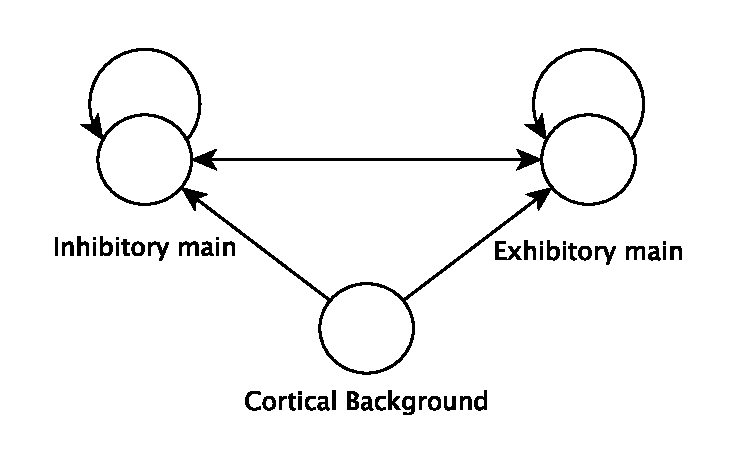
\includegraphics[width=0.99\textwidth]{twoPopNetwork.eps}
    \label{fig:twoPopNetwork}
    \caption{The network of the two population network simulation.}
\end{figure}

\begin{figure}[tbp]
	\begin{subfigure}[b]{0.48\linewidth}
		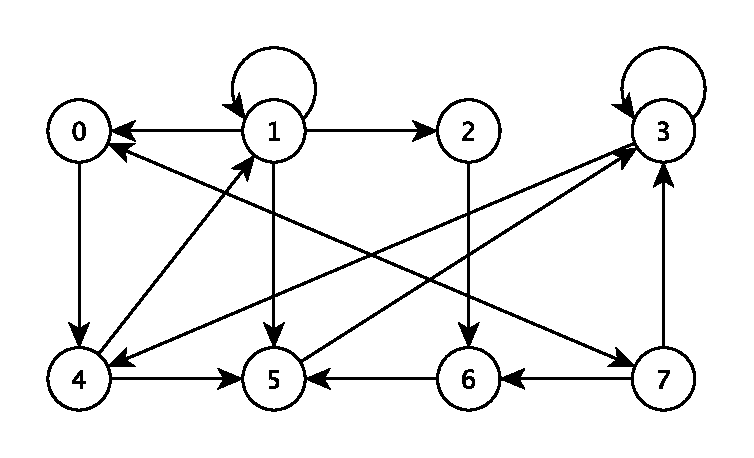
\includegraphics[width=0.99\textwidth]{realNetwork.eps}
        \caption{An example network representation. The circles correspond to the neurons and the arrows between them to directed connection between them.}
		\label{fig-realNetwork}
	\end{subfigure} 
	\quad
	\begin{subfigure}[b]{0.48\linewidth}
		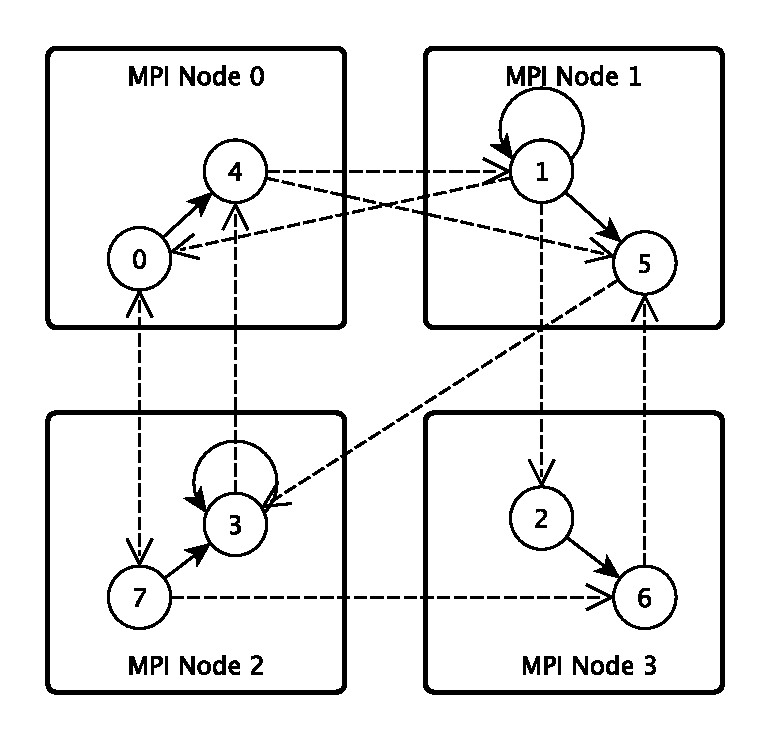
\includegraphics[width=0.99\textwidth]{internalNetwork.eps}
        \subcaption{The internal representation of the network. The circles correspond to the neurons. The rounded boxes represent the individual MPI Nodes. For the distribution the default circular distribution was used. The dashed arrows correspond to asynchronous MPI messages. The normal arrows correspond to internal messages.}
		\label{fig-internalNetwork}
	\end{subfigure}
    \caption{The real and internal representation of a small network.}
\end{figure}


\end{document}

